\section{Introduction}

\begin{frame}{Motivation}
    By definition, intelligence is the ability to derive information, learn from experience, adapt to the environment, understand, and correctly utilize thought and reason~\cite{chollet2019measure}.\\
    \vspace{0.5cm}
    \begin{figure}[!htb]
        \centering
        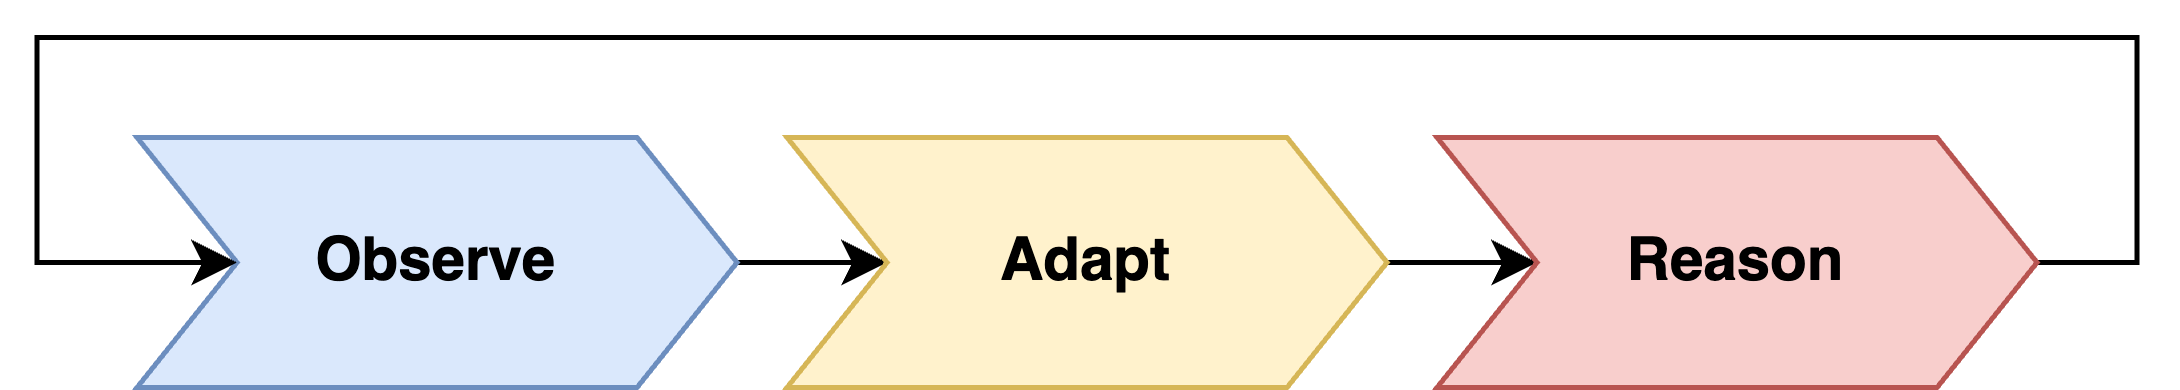
\includegraphics[width=0.8\textwidth]{img/intelligence}
        \captionsetup{font=small,labelformat=empty}
        \caption{Three components of intelligence.}
    \end{figure}
    So what if we can create a machine that can do all of that?
\end{frame}

\begin{frame}{Motivation}
    \begin{figure}[!htb]
        \centering
        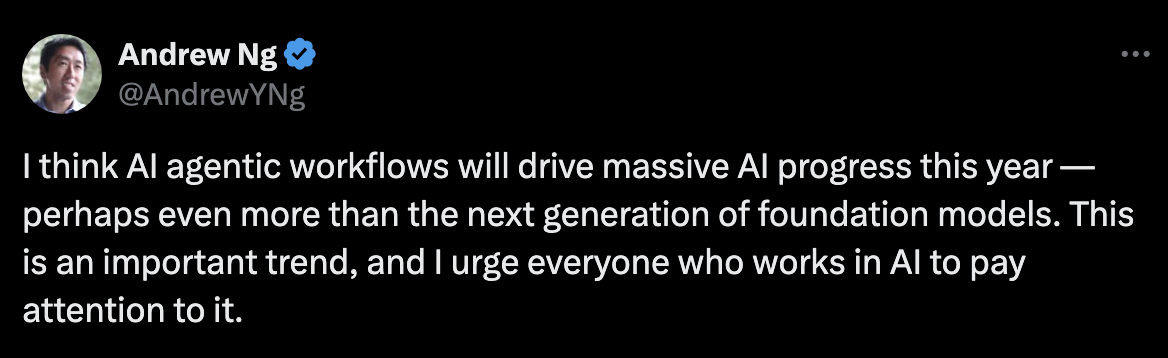
\includegraphics[width=1.0\textwidth]{img/agentic_workflow}
        \captionsetup{font=small,labelformat=empty}
        \caption{Andrew Ng on Agentic Workflows.\footnotemark[1]}
    \end{figure}
    \footnotetext[1]{\footnotesize https://twitter.com/AndrewYNg/status/1770897666702233815}
\end{frame}
